%! TeX program = lualatex
\documentclass[../main.tex]{subfiles}
\begin{document} \section{Equilibria and their stability}

Recall (from the very first lecture of the semester) that models are \emph{imperfect} representations of natural phenomena. Exact solutions to differential equations may or may not be what we \emph{need}.  

We introduce the idea of phase-line plots using the logistic equation. 

\begin{example}[equilibria of logistic equations] \label{eq:diff-eq-logistic-equation-equilibria}
  Consider \(N'(t) = N(t) \left( 1 - \frac{N'(t)}{K} \right)\).

  Notice \(t\) does not appear in the right-hand side of the logistic equation at all. Recall from page~\pageref{def:autonomous} that such an equation is called \hlmain{autonomous}. This is rather special because it allows us to plot \(N\) versus \(N'\) by using \(N\) as an input to produce a value for \(N'\).

  \begin{figure}[H] % [h] for here, [ht] for here top, [hb] for here bottom
    \centering
    \includegraphics{../standalones/build/plot-logistic-solutions-phase-lines}
    \caption{\(N\) versus \(N'\) plot.}
    \label{fig:logistic-solutions-phase-lines}
  \end{figure}

  \faStar{} The above graph \hlmain{predicts} that if a solution curve 
  \begin{itemize}
    \item \underline{\hspace{2in}}, then the solution \underline{\hspace{3in}}.
    \item \underline{\hspace{2in}}, then the solution \underline{\hspace{3in}}.
  \end{itemize}

  This prediction is easily obtained, because we do not need to solve the differential equation.

  Does the above prediction match reality? Here are several solution curves for the logistic equation.
  \begin{figure}[H] % [h] for here, [ht] for here top, [hb] for here bottom
    \centering
    \includegraphics{../standalones/build/plot-logistic-solutions}
    \label{fig:logistic-solutions}
  \end{figure}

\end{example}

The punchline of this example is that such predictions can be made reliably for all autonomous equations.  Plots like Figure~\ref{fig:logistic-solutions-phase-lines} are called phase-line plots.

\clearpage

Creating a phase-line plot is really a job for the computer. We will do more of that when discussing scientific computing.

For the rest of the section, we learn the concept of stability of equilibria.

\begin{definition}[stability of equilibria]
  Suppose we have an \emph{autonomous} differential equation in which \(u\) is the unknown function. 

  Equilibria of the autonomous differential equation shows up as zeros of the phase-line plot.

  \begin{itemize}
    \item If the phase-line plot is \hlmain{above} the horizontal axis (the \(u\)-axis) to the left of \(\bar{u}\) and \hlsupp{below} the horizontal axis to the right of \(\bar{u}\), then \(\bar{u}\) is called a \hlmain{locally asymptotically stable} equilibrium.
    \item If the phase-line plot is \hlsupp{below} the horizontal axis (the \(u\)-axis) to the left of \(\bar{u}\) and \hlmain{above} the horizontal axis to the right of \(\bar{u}\), then \(\bar{u}\) is called a \hlmain{locally asymptotically unstable} equilibrium.
  \end{itemize}
\end{definition}

% \faStar{} We \hlsupp{do not need to solve} \emph{autonomous} differential equations to understand \hlmain{how their equilibria affect solutions}.  The idea we need is a slight change of mindset: Treat the dependent variable \(u\) in a differential equation as the independent variable for \(u'\). 

% \begin{definition}[phase-line plots] \label{def:phase-line-plots}
%   Suppose \(u' = g(u)\) is an autonomous differential equation where \(g\) is continuous. The (unknown) dependent variable is \(u\).
%
%   The \hlmain{phase-line plot} of a differential equation is the graph of \(u' = g(u)\) where the vertical axis is \(u'\) and horizontal axis is \(u\).  
%
%   We \hlsupp{do not need to solve} the differential equation at all.
% \end{definition}

\begin{example}
  Consider the following phase-line plot.  Identify its equilibria and their stability.

  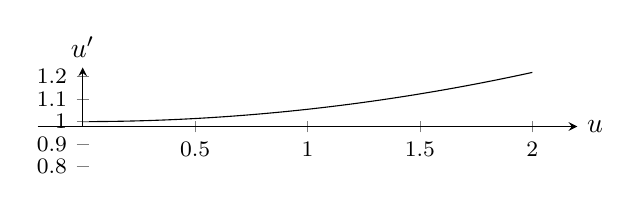
\begin{tikzpicture}
    \begin{axis}[
    axis lines = middle, % boxed, middle
    axis on top,
    axis equal image,
    %
    % domain and range
    %
    % xmin={}, xmax={},
    % ymin={}, ymax={},
    enlargelimits=true,
    %
    % axis labels
    %
    xlabel={\(u\)}, xlabel style={anchor=west},
    ylabel={\(u'\)}, ylabel style={anchor=south},
    label style={at={(ticklabel* cs:1)}},
    %
    % ticks
    %
    % xtick={}, xticklabels={},
    % ytick={}, yticklabels={},
    ticklabel style={font=\footnotesize},
    %
    % grid
    % none, major, minor, both
    grid=none, grid style={gray!20},
    % minor tick num=1, 
    % minor grid style={gray!20},
    % 
    % plot parameters
    %
    smooth, samples=100, no markers,
    ]
    % \usepackage{pgfplots}
    % \pgfplotsset{compat=newest, trig format=rad} 
    % \pgfplotsset{label style={font=\footnotesize}}
    \addplot[domain=0:2] {x*sin(x*pi) + 1};
    \end{axis}
  \end{tikzpicture}
\end{example}


\begin{example}
  Consider the following phase-line plot.  Identify its equilibria and their stability.

  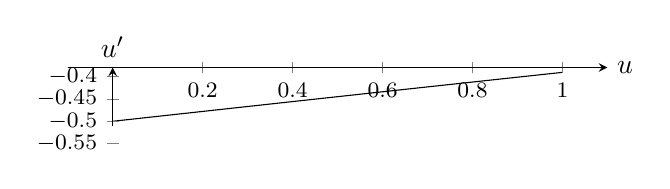
\begin{tikzpicture}
    \begin{axis}[
      axis lines = middle, % boxed, middle
      axis on top,
      axis equal image,
      %
      % domain and range
      %
      % xmin={}, xmax={},
      % ymin={}, ymax={},
      enlargelimits=true,
      %
      % axis labels
      %
      xlabel={\(u\)}, xlabel style={anchor=west},
      ylabel={\(u'\)}, ylabel style={anchor=south},
      label style={at={(ticklabel* cs:1)}},
      %
      % ticks
      %
      % xtick={}, xticklabels={},
      % ytick={}, yticklabels={},
      ticklabel style={font=\footnotesize},
      %
      % grid
      % none, major, minor, both
      grid=none, grid style={gray!20},
      % minor tick num=1, 
      % minor grid style={gray!20},
      % 
      % plot parameters
      %
      smooth, samples=100, no markers,
      ]
      % \usepackage{pgfplots}
      % \pgfplotsset{compat=newest, trig format=rad} 
      % \pgfplotsset{label style={font=\footnotesize}}
      \addplot[domain=0:1] {sin(x*4*pi)/2 - 1/2};
    \end{axis}
  \end{tikzpicture}
\end{example}

What if a computer is not available to create a phase-line plot? We can use qualitative analysis to identify equilibria and their stability.

\begin{example}
  Find equilibria of \(u'(t) = u(t) ( 2 - u(t) )^{2} (3 - u(t)/2)\) and their stability.

  \blanklines{30}

  Evaluate \(\lim_{t \to \infty} u(t)\) given \(u(0) = 1\).  Hint: What did we do in \faStar{} on page \pageref{eq:diff-eq-logistic-equation-equilibria}.
  \blanklines{15}
\end{example}
\clearpage

\begin{example}
  Find the long-term behaviour of the initial-value problem 
  \[
    u'(t) = (u(t) - 3) (2u(t) - 1) (u(t) - 5) \quad\text{and}\quad u(1) = 4.
  \]
  \blanklines{15}
\end{example}


\begin{example}
  Evaluate \(\lim_{t \to \infty} u(t)\) given
  \[
    N'(t) = (N(t) + 1)^{2} (N(t) - 2) (N(t) - 3) \quad\text{and}\quad u(500) = 1.5.
  \]
  \blanklines{15}
\end{example}

\begin{example}
  Consider the differential equation
  \[
    N'(t) = (N(t) - 1) (N(t) - 3) (N(t) - 20)^{3}.
  \]

  Which of the following initial value leads to \(\lim_{t \to \infty} u(t) = 3\)?
  \begin{enumerate}[label=(\alph*)]
    \item \(u(0) = 19\)
    \item \(u(-1) = 21\)
    \item \(u(3) = -1\)
    \item \(u(5) = 1.1\)
  \end{enumerate}
\end{example}

\begin{example}[generate your own exam problem]
  Pick at most \(5\) numbers \(a_{1}, a_{2}, a_{3}, a_{4}, a_{5}\). Duplicates are okay.

  Consider the differential equation
  \[
    u' = (u - a_{1}) (u - a_{2})(u - a_{3})(u - a_{4})(u - a_{5}).
  \]

  Randomly pick a number \(u_{0}\) between \(a_{1}\) and \(a_{5}\).  Ask yourself the following question:
  \begin{enumerate}
    \item What are the equilibria of the differential equation?
    \item What is the long-term behaviour of the solution that satisfies \(u(0) = u_{0}\)?
    \item Plot the phase-line graph to confirm your answer.
  \end{enumerate}
\end{example}
\end{document}
